\documentclass[12pt]{article}

\usepackage[a4paper,margin=2.5cm]{geometry}
\usepackage[T1]{fontenc}
\usepackage[utf8]{inputenc}
\usepackage{lmodern}
\usepackage{microtype}
\usepackage{setspace}
\usepackage{graphicx}
\usepackage{float}
\usepackage{booktabs}
\usepackage{array}
\usepackage{longtable}
\usepackage{enumitem}
\usepackage{xcolor}
\usepackage{listings}
\usepackage{chngcntr}
\usepackage[hidelinks]{hyperref}

\definecolor{codegray}{RGB}{245,245,245}
\definecolor{rulegray}{RGB}{190,190,190}
\setstretch{1.12}
\setlength{\parindent}{0pt}
\setlength{\parskip}{0.6em}
\setlist{itemsep=0.25em,topsep=0.35em}
\renewcommand{\arraystretch}{1.2}
\graphicspath{{resources/}}
\counterwithin{figure}{section}
\lstset{language=bash,basicstyle=\ttfamily\small,backgroundcolor=\color{codegray},frame=single,rulecolor=\color{rulegray},breaklines=true,showstringspaces=false,columns=fullflexible,keepspaces=true,aboveskip=0.8em,belowskip=0.8em}
\newcommand{\cmd}[1]{\texttt{\detokenize{#1}}}
\newcommand{\labimage}[3][0.88\textwidth]{\begin{figure}[H]\centering\includegraphics[width=#1,height=0.68\textheight,keepaspectratio]{\detokenize{resources/#2}}\caption{#3}\end{figure}}

\begin{document}
\pagenumbering{gobble}
\begin{titlepage}
\centering
{\large Ministerul Educației și Cercetării al Republicii Moldova\par}
\vspace{0.45cm}
{\large Universitatea Tehnică a Moldovei\par}
\vspace{0.45cm}
{\large Facultatea Calculatoare, Informatică și Microelectronică\par}
\vspace{0.45cm}
{\large Departamentul Ingineria Software și Automatică\par}
\vspace{3cm}
{\Large\bfseries Report on Laboratory Work No. 4\par}
\vspace{0.55cm}
{\LARGE\bfseries The xv6 Shell from the Outside\par}
\vspace{0.35cm}
{\large Operating Systems\par}
\vfill
\begin{flushleft}
\textbf{Done by:}\\
Student, group FAF-241\\
Caț Chiril\\
\vspace{1cm}
\textbf{Checked by:}\\
asist. univ. Reițman Patricia
\end{flushleft}
\vfill
{Chișinău -- 2026\par}
\end{titlepage}

\pagenumbering{roman}
\tableofcontents
\clearpage
\pagenumbering{arabic}

\section*{Purpose of the Work}
\addcontentsline{toc}{section}{Purpose of the Work}
The purpose of this laboratory is to compare the Bash and xv6 command interpreters through direct experiments, update the xv6 \cmd{sleep} utility for the current system call interface, write argument inspection programs for both environments, and trace the relevant behavior to \cmd{user/sh.c}.

\section*{Environment check}
\addcontentsline{toc}{section}{Environment check}
I read the Linux setup guide and ran \cmd{bash ~/Desktop/os2026-setup.sh --check} in the Ubuntu guest. It confirmed the required tools, found the existing \cmd{~/xv6-riscv} tree, built xv6, booted it, and ran \cmd{ls}. The final status was \cmd{All set}. The RISC-V compiler and QEMU were present. No reinstall was needed.

\begin{center}
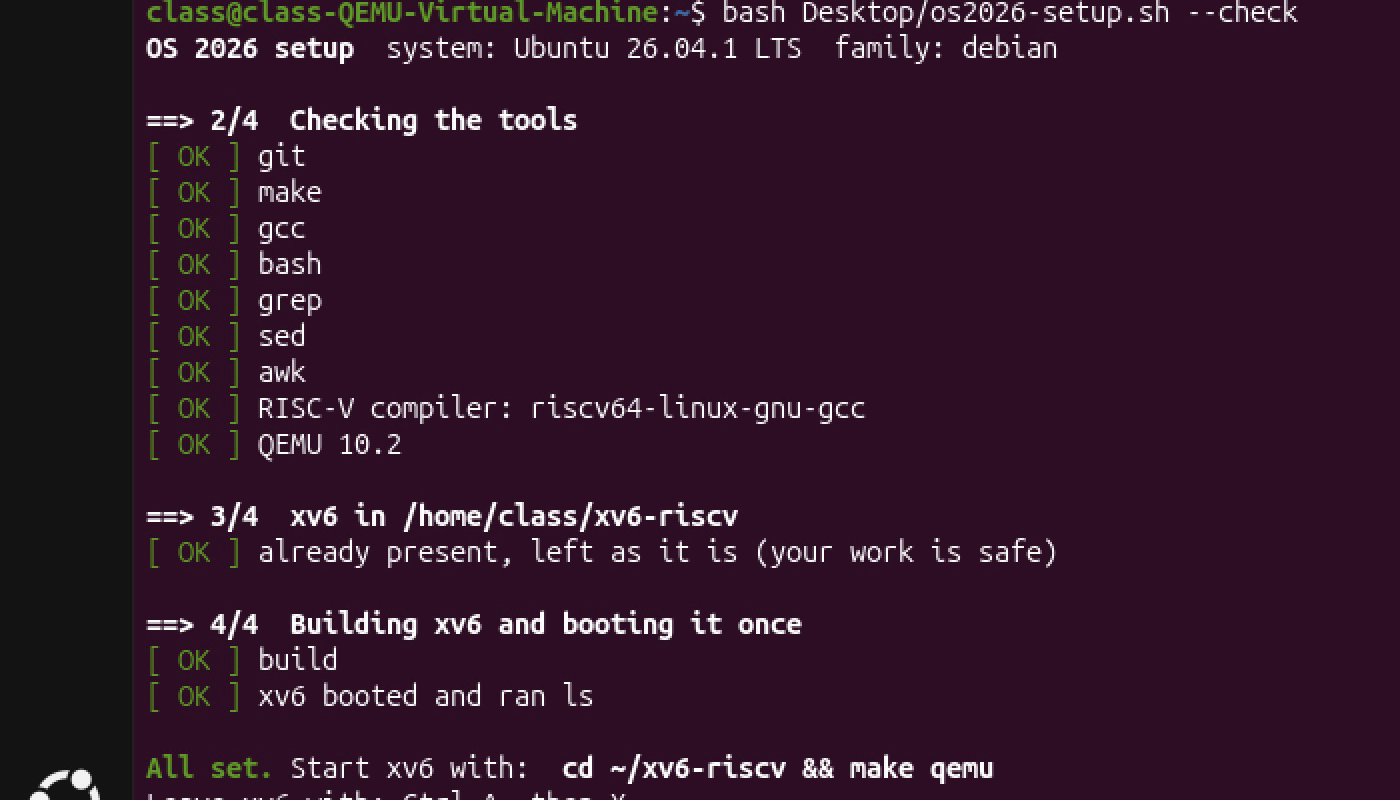
\includegraphics[width=0.88\textwidth,height=0.6\textheight,keepaspectratio]{resources/setup_check_passed_crop.png}\\
{\small Successful setup check in the Ubuntu guest.}
\end{center}

\section{Part 1: Updating the xv6 sleep program}
\cmd{user/user.h} declares \cmd{int pause(int);} on line 25. Accordingly, the xv6 \cmd{sleep} program converts its single argument to ticks and calls \cmd{pause(atoi(argv[1]))}. For a missing argument it prints usage and exits with status 1. The Makefile includes \cmd{$U/_sleep} in \cmd{UPROGS}; the guest build succeeded.

\labimage{figure_1_grep_crop.png}{The \cmd{pause} declaration in \cmd{user/user.h}.}
\labimage{figure_1_sleep_code_crop.png}{Updated \cmd{sleep.c} and its Makefile entry in the guest.}

\begin{lstlisting}
$ sleep 20
$ sleep
usage: sleep <ticks>
\end{lstlisting}
The first command returned to the prompt after its pause; the second took the error path. Both ran in the xv6 shell after \cmd{make qemu}.

\labimage{figure_1_3_sleep_tests_crop.png}{The successful pause and missing-argument test in xv6.}

\section{Part 2: Bash and xv6 shell comparison}
I ran the commands in Bash in a Linux test directory containing \cmd{README} and in the xv6 root directory. The Linux test directory also contained small \cmd{.c} files used in Part 3. The outputs below record the relevant text; xv6's \cmd{ls} additionally prints file type, inode, and size.

\small
\setlength{\tabcolsep}{4pt}
\begin{longtable}{p{0.24\textwidth}p{0.23\textwidth}p{0.23\textwidth}p{0.22\textwidth}}
\toprule
Command / feature & Bash result & xv6 result & Explanation\\
\midrule
\endfirsthead
\toprule Command / feature & Bash result & xv6 result & Explanation\\ \midrule
\endhead
\cmd{echo hello > f ; cat < f} & \cmd{hello} & \cmd{hello} & Both support redirection and sequencing.\\
\cmd{ls | grep READ} & \cmd{README} & \cmd{README} with metadata & Both create a pipe.\\
\cmd{(echo a; echo b) | wc} & \cmd{2 2 4} & \cmd{2 2 4} & Grouping, list, and pipe work.\\
\cmd{echo one ; echo two} & \cmd{one}, then \cmd{two} & Same & Semicolon executes a list.\\
\cmd{echo bg &} & \cmd{bg} (background job) & \cmd{bg}; prompt can interleave & Both launch a background command.\\
\cmd{ls *} & Lists matched names, including \cmd{README} & \cmd{ls: cannot open *} & Bash expands the wildcard; xv6 passes it literally.\\
\cmd{echo $HOME} & \cmd{/home/class} & Literal \cmd{$HOME} & Bash expands variables.\\
\cmd{echo "a b"} & \cmd{a b} & Literal \cmd{"a b"} & Bash removes quotes and keeps one argument; xv6 does neither.\\
\cmd{mkdir d ; cd d ; ls ..} & Parent names displayed & \cmd{exec ls failed} after \cmd{cd d} & Bash finds \cmd{ls} through \cmd{PATH}; xv6 searches the current directory.\\
Up arrow, Tab, Ctrl+R & History and completion & No corresponding line editing & Bash provides interactive editing.\\
\bottomrule
\end{longtable}
\setlength{\tabcolsep}{6pt}
\normalsize

The shared features are execution, input/output redirection, pipelines, command lists, grouping, background execution, and \cmd{cd}. Bash adds filename globbing, variable expansion, useful quoting, \cmd{PATH} lookup, history, and completion. In the Bash run, \cmd{echo $HOME} returned \cmd{/home/class}; \cmd{echo "a b"} returned \cmd{a b}. The guest transcript is preserved in \cmd{lab4-results.txt}.

\labimage{figure_2_2_xv6_pipes_crop.png}{Pipelines and command lists working in xv6.}
\labimage{figure_2_2_xv6_missing_features_crop.png}{The xv6 shell passes the wildcard, variable name, and quotes literally.}

After \cmd{cd d}, xv6 attempts to execute \cmd{ls} relative to \cmd{d}, where that program is absent. The executable is in the parent (root) directory, so \cmd{../ls} succeeds. Bash uses its \cmd{PATH} to find \cmd{ls} after a directory change.

\labimage{figure_2_3_xv6_path_crop.png}{\cmd{ls} failing from \cmd{d} and \cmd{../ls} succeeding.}

I would miss history and completion most in daily use because they save repeated typing. A limited single-entry history recall would be the easiest feature to add: it only needs to store and replay the last input line. General quoting or globbing needs parser changes and filename expansion.

\section{Part 3: Who expands arguments?}
I wrote \cmd{args.c} for xv6 and \cmd{args_linux.c} for Linux. Each prints \cmd{argc} and every \cmd{argv} element. The xv6 Makefile includes \cmd{$U/_args}. I compiled the Linux version with \cmd{gcc -o args args_linux.c}; \cmd{make} built the xv6 version.

\begin{lstlisting}[language=C,caption={Core of the two argument inspection programs.}]
printf("argc = %d\n", argc);
for(int i = 0; i < argc; i++)
  printf("argv[%d] = [%s]\n", i, argv[i]);
\end{lstlisting}

The decisive command was \cmd{args *.c "x y"}. The Linux directory contained three C files: \cmd{a.c}, \cmd{args_linux.c}, and \cmd{b.c}. Bash produced:
\begin{lstlisting}
argc = 5
argv[0] = [/home/class/args]
argv[1] = [a.c]
argv[2] = [args_linux.c]
argv[3] = [b.c]
argv[4] = [x y]
\end{lstlisting}
In xv6 the same line produced:
\begin{lstlisting}
argc = 4
argv[0] = [args]
argv[1] = [*.c]
argv[2] = ["x]
argv[3] = [y"]
\end{lstlisting}

Thus Bash passed four user arguments, while xv6 passed three. The shell, rather than the program or kernel, expands \cmd{*.c} and processes quotes. The program receives only the resulting argument vector.

\labimage{figure_3_2_xv6_args_crop.png}{The xv6 argument printer with ordinary words and the wildcard/quotes test.}
\labimage{figure_3_2_xv6_args_more_crop.png}{The xv6 argument printer with variables and single quotes.}

With \cmd{args one two three}, both received \cmd{argc = 4}; repeated spaces only separate tokens and are not passed inside the arguments. Bash expanded \cmd{$HOME} to \cmd{/home/class} and turned \cmd{'single quoted'} into one argument without quotes. xv6 passed \cmd{$HOME} literally and split the quoted words into two arguments with quote characters retained.

\section{Part 4: Reading \cmd{user/sh.c}}
The guest's \cmd{user/sh.c} has 499 lines. Its command tags are defined near the top and dispatched in \cmd{runcmd}:

\begin{center}
\begin{tabular}{lll}
\toprule
Tag & Input syntax & Action\\
\midrule
\cmd{EXEC} & a program name (no operator) & Execute a program.\\
\cmd{REDIR} & \cmd{<}, \cmd{>}, \cmd{>>} & Redirect a file descriptor.\\
\cmd{PIPE} & \cmd{|} & Connect two commands by pipe.\\
\cmd{LIST} & \cmd{;} & Run commands in sequence.\\
\cmd{BACK} & \cmd{&} & Run without waiting in the foreground.\\
\bottomrule
\end{tabular}
\end{center}

\begin{lstlisting}
8:#define EXEC  1       75:  case EXEC:
9:#define REDIR 2       83:  case REDIR:
10:#define PIPE  3       101: case PIPE:
11:#define LIST  4       93:  case LIST:
12:#define BACK  5       125: case BACK:
\end{lstlisting}

The \cmd{cd} check is in the shell's main input loop, around lines 164--172, before the usual fork and command execution. Changing directory must affect the shell process itself. If \cmd{cd} ran as a separate child program, only that child's working directory would change; the next prompt would still be in the old directory.

\begin{lstlisting}[language=C]
char *cmd = buf;
while (*cmd == ' ' || *cmd == '\t')
  cmd++;
if (cmd[0] == 'c' && cmd[1] == 'd' && cmd[2] == ' ') {
  cmd[strlen(cmd) - 1] = 0;
  if (chdir(cmd + 3) < 0)
    fprintf(2, "cannot cd %s\n", cmd + 3);
} else {
  if (fork1() == 0)
    runcmd(parsecmd(cmd));
  wait(0);
}
\end{lstlisting}

The parser has no wildcard or variable-expansion stage. It treats \cmd{*} and \cmd{$} as ordinary word characters. This explains the literal \cmd{ls *} failure and the \cmd{$HOME} output in Part 2. The shell also lacks Bash-style quote processing, matching the Part 3 argument results.

\section*{Conclusions}
\addcontentsline{toc}{section}{Conclusions}
The environment check, xv6 build, and boot completed successfully. Updating \cmd{sleep} to call \cmd{pause} made it work with this tree. Direct shell tests showed that xv6 supports the core execution operators but lacks the expansion and interactive conveniences of Bash. The argument printers established that expansion and quote handling occur in the shell before a program starts. Reading \cmd{sh.c} connected those observations to its five command types and its special handling of \cmd{cd}.

\end{document}
